\documentclass[totpages,helvetica,openbib,italian]{europecv}
\usepackage[T1]{fontenc}
\usepackage{graphicx}
\usepackage[a4paper,top=1.27cm,left=1cm,right=1cm,bottom=2cm]{geometry}
\usepackage[italian]{babel}
\usepackage{bibentry}
\usepackage{url}
\usepackage{enumitem}
\setlist{nolistsep}

\renewcommand{\normalsize}{\fontsize{2.9mm}{3.1mm}\selectfont}

\ecvname{Diego Russo}
\ecvaddress{Via G. Garibaldi 40, 05021, Acquasparta (TR), Italia}
\ecvtelephone[+39 334 5873886]{+39 0744 930614}
\ecvemail{\url{diegor.it@gmail.com} - Personale, gtalk, MSN \\& \url{diego.russo@forinicom.it} - Forinicom S.r.l.}
\ecvhomepage{\url{http://www.diegor.it}}
\ecvnationality{Italiana}
\ecvdateofbirth{30 aprile 1983}
\ecvgender{Maschio}
\ecvbeforepicture{\raggedleft}
\ecvpicture[width=3cm]{diegor.jpg}
\ecvafterpicture{\ecvspace{-3cm}} 
\ecvfootnote{Per ulteriori informazioni: \url{http://europass.cedefop.eu.int}\\
\textcopyright~European Communities, 2003.}

\begin{document}
    \begin{center}
        \hspace{1pt}
        \vspace{2cm}
    
        {\scshape \textbf{\Huge Diego Russo}}
    
        \vspace{1cm}
    
        {\scshape \textbf{\large \underline{Curriculum Vitae}}}
    
        \vspace{0.25cm}
    
        aggiornato al \emph{\textbf{10 marzo 2010}}
        
        \vspace{2cm}
        
        \begin{figure}[htbp] 
            \begin{center} 
                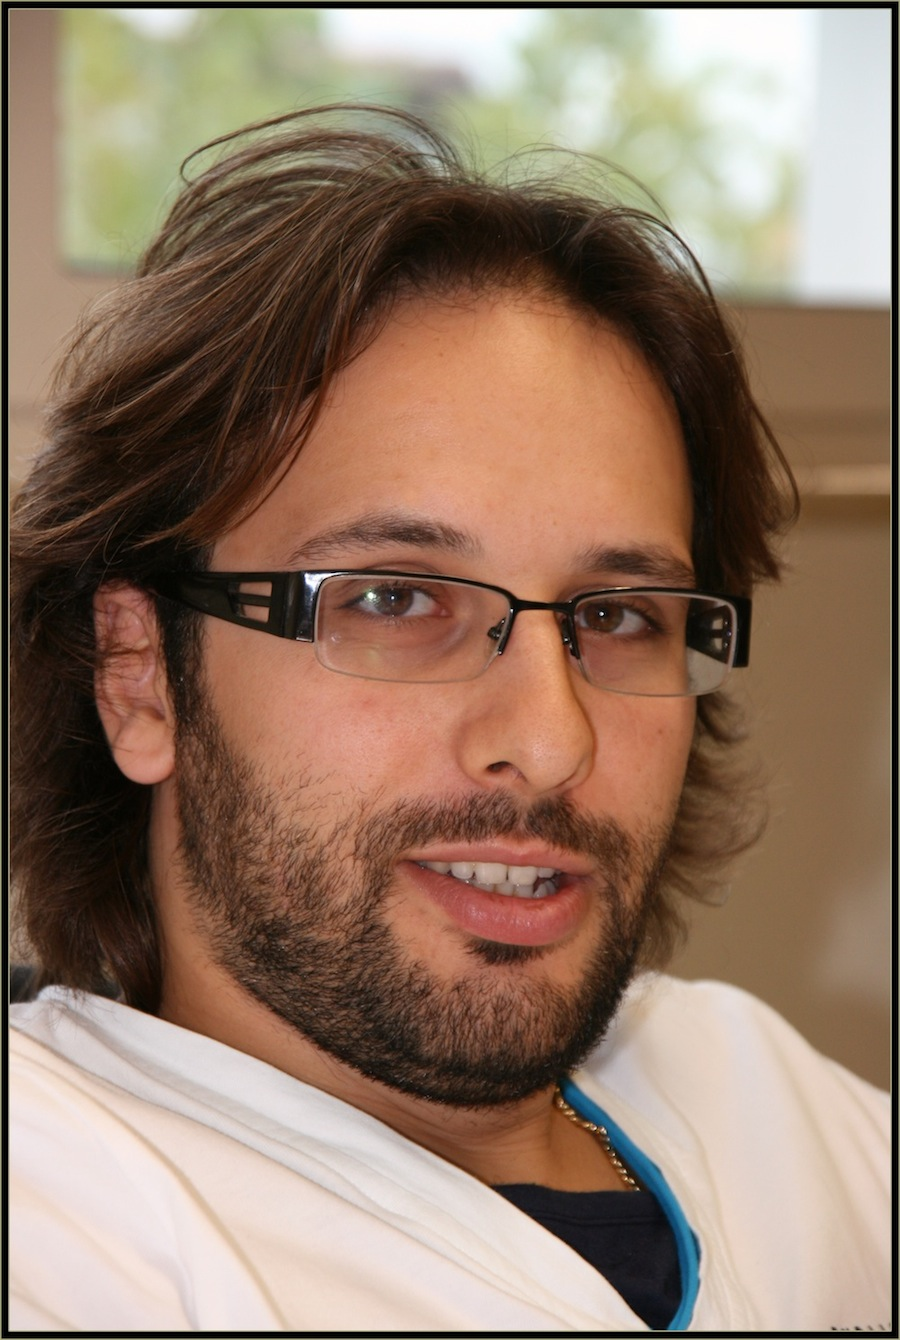
\includegraphics[width=10cm]{io.jpg}
            \end{center} 
        \end{figure}
        
    \end{center}
\pagebreak
\selectlanguage{italian}

\begin{europecv}
\ecvpersonalinfo[5pt]

\ecvitem{\large\textbf{Impiego ricercato/ Settore di competenza}}{\large\textbf{Programmatore Python, Django. Sistemista Linux, OSX. Aperto anche ad altre proposte con possibilit\'a di crescita professionale e personale.}}

\ecvsection{Esperienza professionale}

\ecvitem{Date}{\textbf{Dal 26 aprile 2008 ad Oggi}}
\ecvitem{Lavoro o posizione ricoperti}{Programmatore, sistemista (lavoratore con contratto di apprendistato part-time, 25 ore)}
\ecvitem{Principali attivit\'a e responsabilit\`a}{Sviluppo di un progetto che mira ad offrire connettivit\'a e servizi integrati (videosorveglianza, voip) alle pubbliche amministrazioni, aziende e privati. Punti previsti dal contratto:
\begin{itemize}
    \item conoscere i prodotti ed i servizi del settore e del contesto aziendale: reti Mesh e gararchiche, servizi VoIP e videosorveglianza, sicurezza delle reti wired e wireless;
    \item conoscere e saper applicare le basi tecniche e scientifiche della professionalit\'a;
    \item conoscere e saper utilizzare tecniche e metodi di lavoro con particolare riferimento allo sviluppo software e alla documentazione del codice;
    \item conoscere e saper utilizzare strumenti e tecnologie di lavoro (attrezzature, macchinari e strumenti di lavoro), in particolare ambiente di sviluppo Linux, piattaforma di sviluppo Linux/OSX, linguaggi di programmazione Python e database PostgresSQL/MySQL;
    \item conoscere ed utilizzare misure di sicurezza individuale e per la tutela ambientale;
    \item conoscere le innovazioni di prodotto, di processo, di contesto e di settore.
\end{itemize}
Inoltre ho sviluppato applicazioni in python e in python-django sia per il lavoro quotidiano del reparto tecnico e non sia di pura ricerca e sviluppo. A tal senso ho implementato da zero un server per gestire il \textbf{servizio di hotspot}.}
\ecvitem{Nome e indirizzo del datore di lavoro}{Forinicom srl, Via del Popolo, 9 Bastia Umbra, 06083, 0758001868, \url{http://www.forinicom.it}}
\ecvitem[10pt]{Tipo di attivit\`a o settore}{Settore telecomunicazioni}

\ecvitem{Date}{\textbf{Dal 03 settembre 2009 ad Oggi}}
\ecvitem{Lavoro o posizione ricoperti}{Programmatore (lavoratore con contratto a progetto, part-time)}
\ecvitem{Principali attivit\'a e responsabilit\`a}{Sviluppo di un'applicazione gestionale per il comune di Bettona in django, python, postgresql, linux, apache, per l'informatizzazione dei servizi per la gestione delle anagrafiche nonch\'e delle pratiche edilizie ed urbanistiche e del calcolo della tassa ICI con aggiornamenti dei dati catastali. Utilizzo di un server per il controllo di versione (GIT). Inoltre in questa fase c'\'e stata il completamento del prodotto con la relativa commercializzazione.}
\ecvitem{Nome e indirizzo del datore di lavoro}{Consorzio Miles - Servizi Integrati, CF 04881101002, Via Rocca di Papa 21, Roma}
\ecvitem[10pt]{Tipo di attivit\`a o settore}{Servizi integrati per la pubblica amministrazione}

\ecvitem{Date}{\textbf{Dal 01 agosto 2007 al 31 agosto 2008}}
\ecvitem{Lavoro o posizione ricoperti}{Programmatore (lavoratore con contratto a progetto, full-time)}
\ecvitem{Principali attivit\'a e responsabilit\`a}{Sviluppo di un'applicazione gestionale per il comune di Bettona in django, python, postgresql, linux, apache, per l'informatizzazione dei servizi per la gestione delle anagrafiche nonch\'e delle pratiche edilizie ed urbanistiche e del calcolo della tassa ICI con aggiornamenti dei dati catastali. Utilizzo di un server per il controllo di versione (SVN), con relativa interfaccia web (trac) per la gestione dei ticket.}
\ecvitem{Nome e indirizzo del datore di lavoro}{Consorzio Miles - Servizi Integrati, CF 04881101002, Via Rocca di Papa 21, Roma}
\ecvitem[10pt]{Tipo di attivit\`a o settore}{Servizi integrati per la pubblica amministrazione}

\ecvitem{Date}{\textbf{Dal 11 dicembre 2006 al 30 luglio 2007}}
\ecvitem{Lavoro o posizione ricoperti}{Programmatore (lavoratore con contratto a progetto, full-time)}
\ecvitem{Principali attivit\'a e responsabilit\`a}{Sviluppo di un'applicazione gestionale per il comune di Bettona in django, python, postgresql, linux, apache, per l'informatizzazione dei servizi per la gestione delle anagrafiche nonch\'e delle pratiche edilizie ed urbanistiche e del calcolo della tassa ICI con aggiornamenti dei dati catastali. Utilizzo di un server per il controllo di versione (SVN), con relativa interfaccia web (trac) per la gestione dei ticket.}
\ecvitem{Nome e indirizzo del datore di lavoro}{Consorzio Miles - Servizi Integrati, CF 04881101002, Via Rocca di Papa 21, Roma}
\ecvitem[10pt]{Tipo di attivit\`a o settore}{Servizi integrati per la pubblica amministrazione}

\ecvitem{Date}{\textbf{Dal 30 luglio 2006 al 30 dicembre 2006}}
\ecvitem{Lavoro o posizione ricoperti}{Tesista (Wireless Broadband Network)}
\ecvitem{Principali attivit\'a e responsabilit\`a}{Wireless Broadband Network - progetto \textbf{WeConnect} - Banda larga su reti wireless:
    \begin{itemize}
        \item Ampia conoscenza della rete wireless e del suo funzionamento
        \item Buona conoscenza della normativa che regola il Wi-Fi
        \item Ottima conoscenza del sistema RouterOS (www.mikrotik.com)
        \item Conoscenza del protocollo AAA e del server FreeRADIUS
        \item Amministrazione dei vari servizi di rete: mail (postfix), server web (apache), DNS (pdns), firewall (iptables), database (postgresql), hotspot (chillispot), OS Debian, Voyage (OS per sistemi embedded, basata su Debian)
    \end{itemize}}
\ecvitem{Nome e indirizzo del datore di lavoro}{WEDOIT s.a.s. - Via Protomartiri Francescani,26 - 06088 Assisi (PG)}
\ecvitem[10pt]{Tipo di attivit\`a o settore}{Soluzioni informatiche}

\ecvitem{Date}{\textbf{Dal 14 novembre 2005 al 30 maggio 2006}}
\ecvitem{Lavoro o posizione ricoperti}{Stagista (S.E.O. Search Engine Optimization)}
\ecvitem{Principali attivit\'a e responsabilit\`a}{\vspace{-2mm}
    \begin{itemize}
        \item Conoscenza del SEO e dei sui meccanismi. Ottimizzazione di un sito per il S.E.O.
        \item Tecniche di Pageranking e link popularity
        \item Sistemista di un server virtuale, basato su Debian
        \item Studio del linguaggio di programmazione Python, con l'implementazione di alcune applicazione orientate al S.E.O.
        \item Studio del linguaggio di programmazione PHP, per lo sviluppo di alcune applicazioni orientate al S.E.O.
    \end{itemize}}
\ecvitem{Nome e indirizzo del datore di lavoro}{WEDOIT s.a.s. - Via Protomartiri Francescani,26 - 06088 Assisi (PG)}
\ecvitem[10pt]{Tipo di attivit\`a o settore}{Soluzioni informatiche}

\ecvitem{Date}{\textbf{Marzo 2002}}
\ecvitem{Lavoro o posizione ricoperti}{Stagista (Stage abbinato al progetto IFS, Impresa Formativa Simulata)}
\ecvitem{Principali attivit\'a e responsabilit\`a}{Gestione della rete interna dell'impresa}
\ecvitem{Nome e indirizzo del datore di lavoro}{IOSA CARLO S.r.l. - 05100 TERNI - Via Pallotta n. 7 - Tel. (0744) 2460 - Fax (0744) 246035 - P.IVA 00072550551 - \url{http://www.iosacarlo.com} - \url{iosacarlo@iosacarlo.com}}
\ecvitem[10pt]{Tipo di attivit\`a o settore}{Impresa smaltimento rifiuti}

\ecvsection{Istruzione e formazione}

\ecvitem{Date}{\textbf{Da Ottobre 2008 a oggi}}
\ecvitem{Titolo della qualifica rilasciata}{Iscritto alla specializzazione di Informatica, indirizzo di ``Sicurezza Informatica''}
\ecvitem{Principali tematiche/competenze professionali possedute}{Sostenuti i seguenti esami con relativa votazione:\begin{itemize}
    \item Simulazione: 30 e lode
    \item Programmazione Avanzata: 30 e lode
    \item Sistemi operativi avanzati: 30 e lode
    \item Laboratorio di Sistemi operativi avanzati: 30 e lode
\end{itemize}}
\ecvitem{Nome e tipo d'organizzazione erogatrice dell'istruzione e formazione}{Universit\'a degli studi di Perugia, Dipartimento di Informatica}
\ecvitem[10pt]{Livello nella classificazione nazionale o internazionale}{-}

\ecvitem{Date}{\textbf{Dal 17 Febbraio 2010 ad Oggi}}
\ecvitem{Titolo della qualifica rilasciata}{Iscritto al 4$^\circ$ modulo di lingua spagnola}
\ecvitem{Principali tematiche/competenze professionali possedute}{I livelli raggiunti in questo modulo sono i seguenti:
\begin{itemize}
    \item capire gli elementi principali in un discorso chiaro in lingua standard su argomenti familiari
    \item riuscire a descrivere esperienze ed avvenimenti, motivare e spiegare progetti
    \item affrontare molte delle situazioni che si possono presentare viaggiando in una zona dove si parla la lingua
\end{itemize}}
\ecvitem{Nome e tipo d'organizzazione erogatrice dell'istruzione e formazione}{Istituto comprensivo ``Volumnio'' Ponte San Giovanni - Perugia}
\ecvitem[10pt]{Livello nella classificazione nazionale o internazionale}{-}

\ecvitem{Date}{\textbf{Da Agosto 2009 a Marzo 2010}}
\ecvitem{Titolo della qualifica rilasciata}{Pubblicazione del paper \textbf{``The AES implentation based on OpenCL for multi/many core architecture''}}
\ecvitem{Principali tematiche/competenze professionali possedute}{Preparazione e pubblicazione del paper ``The AES implentation based on OpenCL for multi/many core architecture'' per l'annuale conferenza ICCSA 2010 (\url{www.iccsa.org}) alla Sangyo University, Fukuoka in Giappone. Il paper tratta di una implementazione di AES eseguito su core GPU NVIDIA/ATI.}
\ecvitem{Nome e tipo d'organizzazione erogatrice dell'istruzione e formazione}{Universit\'a degli studi di Perugia, Dipartimento di Informatica}
\ecvitem[10pt]{Livello nella classificazione nazionale o internazionale}{-}

\ecvitem{Date}{\textbf{Dal 14 Ottobre 2009 al 12 Febbraio 2010}}
\ecvitem{Titolo della qualifica rilasciata}{Attestato di frequenza di 42 ore su 50 del 3$^\circ$ modulo di lingua spagnola}
\ecvitem{Principali tematiche/competenze professionali possedute}{I livelli raggiunti in questo modulo sono i seguenti:
\begin{itemize}
    \item comprendere frasi ed espressioni di uso frequente relativi ad ambiti di immediata rilevanza
    \item saper descrivere in termini semplici aspetti della propria storia e delle proprie esperienze
    \item saper parlare dell'ambiente circostante e saper esprimere bisogni, intenzioni e previsioni
\end{itemize}}
\ecvitem{Nome e tipo d'organizzazione erogatrice dell'istruzione e formazione}{Istituto comprensivo ``Volumnio'' Ponte San Giovanni - Perugia}
\ecvitem[10pt]{Livello nella classificazione nazionale o internazionale}{-}

\ecvitem{Date}{\textbf{Da agosto 2007 a agosto 2008}}
\ecvitem{Titolo della qualifica rilasciata}{Pubblicazione del libro \textbf{UbuntuSemplice 7.10} con conseguente donazione a Canonical Ltd.}
\ecvitem{Principali tematiche/competenze professionali possedute}{\vspace{-2mm}
\begin{itemize}
    \item Contributor, autore di molti capitoli e sistemista del sistema informatico per \url{http://www.ubuntusemplice.org/}
    \item Amministrazione di un server virtuale Debian
    \item Configurazione ed utilizzo del software collaborativo MediaWiki per la stesura e composizione del libro.
    \item Configurazione del server web apache
    \item Configurazione di una mailing list per la gestione dei capitoli del libro con gli altri contributor
\end{itemize}}
\ecvitem{Nome e tipo d'organizzazione erogatrice dell'istruzione e formazione}{Progetto Ubuntusemplice - \url{http://www.ubuntusemplice.org/)}}
\ecvitem[10pt]{Livello nella classificazione nazionale o internazionale}{Ottima conoscenza del sistema operativo Ubuntu}

\ecvitem{Date}{\textbf{Da febbraio 2007 a luglio 2007}}
\ecvitem{Titolo della qualifica rilasciata}{Patente di operatore di stazione di radioamatore di classe A}
\ecvitem{Principali tematiche/competenze professionali possedute}{Corso per aspiranti radioamatori:
\begin{itemize}
    \item Ottima conoscenza delle basi della radiotecnica
    \item Ottima conoscenza delle apparecchiature radio e del loro funzionamento
    \item Conoscenza delle basi della fisica e chimica (magnetismo,  elettromagnetismo)
\end{itemize}}
\ecvitem{Nome e tipo d'organizzazione erogatrice dell'istruzione e formazione}{C.I.S.A.R. Sezione di Foligno}
\ecvitem[10pt]{Livello nella classificazione nazionale o internazionale}{IDONEO, Nominativo internazionale \textbf{IZ0OVB}}

\ecvitem{Date}{\textbf{Dal 19 marzo 2007 al 23 marzo 2007}}
\ecvitem{Titolo della qualifica rilasciata}{Attestato di partecipazione al corso di lingua spagnola}
\ecvitem{Principali tematiche/competenze professionali possedute}{\vspace{-2mm}
\begin{itemize}
    \item Grammatica di base della lingua spagnola
    \item Cultura generale spagnola
\end{itemize}}
\ecvitem{Nome e tipo d'organizzazione erogatrice dell'istruzione e formazione}{Inhispania Intlance S.L / CIF:B83744847 , Montera 10-12, 1-1. 28013, Madrid (Spain)}
\ecvitem[10pt]{Livello nella classificazione nazionale o internazionale}{Valutazioni\footnote{Valutazione in accordo con il ``Common European Framework of Reference for Languages''}:
\begin{itemize}
    \item Espressione orale: A2
    \item Espressione scritta: A2
    \item Comprensione orale: A2
    \item Comprensione scritta: A2
    \item Interazione orale: A2
\end{itemize}}

\ecvitem{Date}{\textbf{03-10-25 Marzo 2007}}
\ecvitem{Titolo della qualifica rilasciata}{Attestato di partecipazione al corso su tecnologie Microsoft}
\ecvitem{Principali tematiche/competenze professionali possedute}{Gli argomenti trattati al corso sono stati:
\begin{itemize}
    \item .NET Framework Architeture (2.0)
    \item ADO.NET
    \item ASP.NET (web forms, Page, controlli, sicurezza)
    \item C\#
    \item Web Service
    \item Ajax.net
    \item Microsoft Visual Studio 2005
\end{itemize}}
\ecvitem{Nome e tipo d'organizzazione erogatrice dell'istruzione e formazione}{O.S.MO.S.IT, Via Strozzacapponi, 85, 06071 Castel del Piano (Pg)}
\ecvitem[10pt]{Livello nella classificazione nazionale o internazionale}{Conoscenza di base della programmazione Microsoft}

\ecvitem{Date}{\textbf{Da settembre 2006 a febbraio 2007}}
\ecvitem{Titolo della qualifica rilasciata}{Pubblicazione del libro \textbf{UbuntuSemplice 6.06} con conseguente donazione a Canonical Ltd.}
\ecvitem{Principali tematiche/competenze professionali possedute}{\vspace{-2mm}
\begin{itemize}
    \item Contributor, autore di molti capitoli e sistemista del sistema informatico per \url{http://www.ubuntusemplice.org/}
    \item Amministrazione di un server virtuale Debian
    \item Configurazione ed utilizzo del software collaborativo MediaWiki per la stesura e composizione del libro.
    \item Configurazione del server web apache
    \item Configurazione di una mailing list per la gestione dei capitoli del libro con gli altri contributor
\end{itemize}}
\ecvitem{Nome e tipo d'organizzazione erogatrice dell'istruzione e formazione}{Progetto Ubuntusemplice - \url{http://www.ubuntusemplice.org/)}}
\ecvitem[10pt]{Livello nella classificazione nazionale o internazionale}{Ottima conoscenza del sistema operativo Ubuntu}

\ecvitem{Date}{\textbf{01-02-03 Dicembre 2006}}
\ecvitem{Titolo della qualifica rilasciata}{Attestato di partecipazione al corso sulle certificazioni ISO}
\ecvitem{Principali tematiche/competenze professionali possedute}{Corso di formazione sulla sicurezza e certificazioni ISO:
\begin{itemize}
    \item ISO 27001:2005
    \item Politica per la sicurezza delle informazioni
    \item Analisi dei rischi (RA)
    \item Analisi dei controlli della ISO 17799:2005
    \item Trattamento dei rischi (RTP)
    \item Processo di certificazione
    \item Panorama delle certificazioni esistenti per gli audit
    \item Piano di audit e checklist
    \item Rapporto di audit
    \item Uno sguardo alle future certificazioni
\end{itemize}}
\ecvitem{Nome e tipo d'organizzazione erogatrice dell'istruzione e formazione}{WEDOIT s.a.s. - Via Protomartiri Francescani, 26 - 06088 Assisi (PG)}
\ecvitem[10pt]{Livello nella classificazione nazionale o internazionale}{Conoscenza dei processi di certificazione ISO}

\ecvitem{Date}{\textbf{Da ottobre 2002 a Novembre 2006}}
\ecvitem{Titolo della qualifica rilasciata}{\textbf{Laurea triennale (nuovo ordinamento) in Informatica}}
\ecvitem{Principali tematiche/competenze professionali possedute}{Laurea triennale in informatica, \textbf{indirizzo ``Reti di computer''}:
\begin{itemize}
    \item Matematica (analitica e discreta)
    \item Programmazione (C, Java, Php, html, xml, xsl, dtd, Pascal, scripting bash e csh, VB.NET, VRML)
    \item DataBase (Mysql, MS Access e loro interazioni con liguaggi di
    \item programmazione)
    \item Reti (ATM, xDSL, Mpls, X.25, Frame Relay), tipologie (wireless, wired) e loro interazione
    \item Conoscenza di sistemi multimediali
    \item Cenni di calcolo parallelo (mpi)
\end{itemize}}
\ecvitem{Nome e tipo d'organizzazione erogatrice dell'istruzione e formazione}{Universit\'a degli studi di Perugia, Dipartimento di Informatica}
\ecvitem[10pt]{Livello nella classificazione nazionale o internazionale}{\textbf{102/110}}

\ecvitem{Date}{\textbf{Da settembre 1996 a giugno 2002}}
\ecvitem{Titolo della qualifica rilasciata}{\textbf{Diploma in ragioniere programmatore (progetto Mercurio)}}
\ecvitem{Principali tematiche/competenze professionali possedute}{Materie previste dal percorso di studio dell'Istituto Tecnico Commerciale, definito dal Ministero dell'Istruzione, ovvero:
\begin{itemize}
    \item Scienze della Materia
    \item Matematica e Laboratorio
    \item Scienze della Natura
    \item Trattamento Testi e Dati
    \item Seconda lingua straniera (Francese)
    \item Diritto ed Economia
    \item Economia Aziendale
    \item Economia Politica e Scienza delle Finanze
    \item Lingua e letteratura italiana
    \item Storia
    \item Informatica Gestionale
    \item Matematica applicata
    \item Prima lingua straniera (Inglese)
    \item Diritto
\end{itemize}}
\ecvitem{Nome e tipo d'organizzazione erogatrice dell'istruzione e formazione}{Ministero della Pubblica Istruzione - I.T.C. ``Federico Cesi'', Terni}
\ecvitem[10pt]{Livello nella classificazione nazionale o internazionale}{\textbf{85/100}}

\ecvitem{Date}{\textbf{Dal 2001 al 2002}}
\ecvitem{Titolo della qualifica rilasciata}{Attestato di frequenza al Progetto Nazionale IFS (\textbf{Impresa Formativa Simulata})}
\ecvitem{Principali tematiche/competenze professionali possedute}{Simulazione di un'impresa di smaltimento rifiuti, affiancati dall'impresa Iosa Carlo S.r.l. (\url{http://www.iosacarlo.com}).
Nell'ambito del progetto ho coordinato il lavoro di tutti gli studenti, realizzando l'organigramma dell'azienda simulata e programmando il sito dell'azienda.}
\ecvitem{Nome e tipo d'organizzazione erogatrice dell'istruzione e formazione}{Ministero della Pubblica Istruzione - I.T.C. ``Federico Cesi'', Terni}
\ecvitem[10pt]{Livello nella classificazione nazionale o internazionale}{-}

\ecvitem{Date}{\textbf{Dal 24 settembre 2001 al 14 ottobre 2001}}
\ecvitem{Titolo della qualifica rilasciata}{Attestato di frequenza al corso come tutor}
\ecvitem{Principali tematiche/competenze professionali possedute}{Svoltasi l'attivit\'a di tutor/referente di un gruppo di altri 6 studenti/tutor, per le attivit\'a di POTENZIAMENTO DI ITALIANO delle prime classi, in ambito del progetto ``Accoglienza, Recupero, Potenziamento nelle Prime Classi''.
L'attivit\'a \'e consistita nell'affiancare i Docenti di Lettere al fine di offrire un valido supporto agli alunni delle Prime Classi nell'utilizzo del Computer, per poter eseguire attivit\'a di approfondimento con il mezzo multimediale, attraverso esercitazioni con un CD-Rom di Grammatica.}
\ecvitem{Nome e tipo d'organizzazione erogatrice dell'istruzione e formazione}{Ministero della Pubblica Istruzione - I.T.C. ``Federico Cesi'', Terni}
\ecvitem[10pt]{Livello nella classificazione nazionale o internazionale}{Acquisite ottime capacit\'a relazionali, organizzative ed ottime competenze nell'insegnamento di materie tecniche}

\ecvitem{Date}{\textbf{Dal 7 dicembre 2001 al 09 dicembre 2001}}
\ecvitem{Titolo della qualifica rilasciata}{Attestato di frequenza del ``Pluto Meeting 2001''}
\ecvitem{Principali tematiche/competenze professionali possedute}{Partecipazione all'organizzazione del ``Pluto Meeting 2001'', tenuto presso il suddetto istituto.}
\ecvitem{Nome e tipo d'organizzazione erogatrice dell'istruzione e formazione}{Ministero della Pubblica Istruzione - I.T.C. ``Federico Cesi'', Terni}
\ecvitem[10pt]{Livello nella classificazione nazionale o internazionale}{-}

\ecvitem{Date}{\textbf{Dal 26 marzo 2001 al 02 aprile 2001}}
\ecvitem{Titolo della qualifica rilasciata}{Attestato di frequenza alla ``XI Settimana della cultura scientifica e tecnologica''}
\ecvitem{Principali tematiche/competenze professionali possedute}{Partecipazione alla ``XI Settimana della cultura scientifica e tecnologica'', realizzando sia la locandina che il programma provinciale della settimana delle scienze in Adobe Photoshop 5.5 ed in Corel Draw 8.0, impegnandosi sia in orario curriculare che extra-curriculare pomeridiano con grande devozione, senso della responsabilit\'a, fungendo anche da punto di riferimento per tutti gli studenti del biennio che hanno partecipato al progetto.}
\ecvitem{Nome e tipo d'organizzazione erogatrice dell'istruzione e formazione}{Ministero della Pubblica Istruzione - I.T.C. ``Federico Cesi'', Terni}
\ecvitem[10pt]{Livello nella classificazione nazionale o internazionale}{-}

\ecvitem{Date}{\textbf{Anno 2001}}
\ecvitem{Titolo della qualifica rilasciata}{Attestato di frequenza come tutor al corso di alfabetizzazione di computer per over 65}
\ecvitem{Principali tematiche/competenze professionali possedute}{Corso di alfabetizzazione di computer di base in funzione di tutor di 40 ore complessive ad un gruppo di 30 persone, con et\'a superiore al 65 anni.
Ho svolto inoltre il ruolo di coordinatore del progetto stilando il programma e coordinando i miei colleghi.}
\ecvitem{Nome e tipo d'organizzazione erogatrice dell'istruzione e formazione}{Ministero della Pubblica Istruzione - I.T.C. ``Federico Cesi'', Terni}
\ecvitem[10pt]{Livello nella classificazione nazionale o internazionale}{-}

\ecvitem{Date}{\textbf{Anno 2001}}
\ecvitem{Titolo della qualifica rilasciata}{Attestato di frequenza al corso di informatica}
\ecvitem{Principali tematiche/competenze professionali possedute}{Corso di informatica di base in funzione di tutor (progetto 20 Studenti) di 30 ore complessive su applicazioni office (Word, Excel) ed Internet}
\ecvitem{Nome e tipo d'organizzazione erogatrice dell'istruzione e formazione}{Ministero della Pubblica Istruzione - I.T.C. ``Federico Cesi'', Terni}
\ecvitem[10pt]{Livello nella classificazione nazionale o internazionale}{-}

\ecvitem{Date}{\textbf{16-17-18 novembre 2000}}
\ecvitem{Titolo della qualifica rilasciata}{Attestato di frequenza all'Exposcuola 2000}
\ecvitem{Principali tematiche/competenze professionali possedute}{Exposcuola - Salone del confronto tra le proposte formative dell'Europa e del Mediterraneo - Paestum hotel Arison}
\ecvitem{Nome e tipo d'organizzazione erogatrice dell'istruzione e formazione}{Ministero della Pubblica Istruzione - I.T.C. ``Federico Cesi'', Terni}
\ecvitem[10pt]{Livello nella classificazione nazionale o internazionale}{-}

\ecvitem{Date}{\textbf{Dal 1997 al 1998}}
\ecvitem{Titolo della qualifica rilasciata}{Attestato di frequenza}
\ecvitem{Principali tematiche/competenze professionali possedute}{Corso di base sulla multimedialit\'a (progetto 20 studenti) per un totale di 25 ore.}
\ecvitem{Nome e tipo d'organizzazione erogatrice dell'istruzione e formazione}{{Ministero della Pubblica Istruzione - I.T.C. ``Federico Cesi'', Terni}}
\ecvitem[10pt]{Livello nella classificazione nazionale o internazionale}{-}

\ecvsection{Capacit\`a e competenze professionali}

\ecvmothertongue[5pt]{Italiana}
\ecvitem{\large Altra/e lingua/e}{\textbf{Inglese, Spagnolo}}
\ecvlanguageheader{(*)}
\ecvlanguage{Inglese}{\ecvBOne}{\ecvBOne}{\ecvATwo}{\ecvATwo}{\ecvBOne}
\ecvlastlanguage{Spagnolo}{\ecvBOne}{\ecvBOne}{\ecvATwo}{\ecvATwo}{\ecvBOne}
\ecvlanguagefooter[10pt]{(*)}

\ecvitem[10pt]{Capacit\`a e competenze sociali}{Ottime capacit\'a di relazionarsi con colleghi e collaboratori, socievole, simpatico con grande capacit\'a di socializzazione e comunicazione. Propenso al lavoro in team. Il mio sito \'e fonte di contatti e scambi sociali continui con altre persone tecniche e meno techiche.)}
\ecvitem[10pt]{Capacit\`a e competenze organizzative}{Capacit\'a di lavorare in maniera efficiente in diverse situazioni.}
\ecvitem[10pt]{Capacit\`a e competenze tecniche ed informatiche}{Vista la mia passione per l'informatica in generale ho sviluppato nell'arco degli anni una serie di competenze che variano in molti settori della stessa.

Fin dal mio primo computer ho avuto una certa passione per il mondo open source e tutto quello che lo riguarda: infatti ho amministrato macchine \textbf{Linux} con varie distribuzioni, come RedHat 7.3, Slackware 7.1 fino ad arrivare a macchine Debian (dalla versione 3.0 a quelle attuali).

Tramite questa esperienza ho maturato una certa abilit\'a e conoscenza nell' aministrazione di Linux: scripting bash, configurazione e compilazione del kernel, servizi di rete, patch per il kernel, linguaggio C. Oltre a Linux uso regolarmente \textbf{OSX}, per l'utilizzo quotidiano. Visto il continuo utilizzo e la mia passione per l'informatica ho approfondito lo studio di OSX, basato su sitemi UNIX.

\textbf{Inoltre ho una certa passione per quanto riguarda la programmazione}: infatti conosco molti linguaggi i ambiti molto diversi tra di loro come Python, C, PHP, java, LSL (Linden Scripting Language). L'LSL l'ho studiato durante la mia attivit\'a su \textbf{Second Life}: infatti ho collaborato su molti progetti italiani presenti nel metaverso come Assisi \url{http://www.secundavita.it}, Milano e Marostica del progetto Italia Vera.
Ho una buona conoscenza di applicazioni grafiche (Gimp, Photoshop)e di strumenti per l'ufficio come Openoffice,org ed iWork (per OSX)}
\ecvitem[10pt]{Capacit\`a e competenze artistiche}{\vspace{-2mm}
\begin{itemize}
    \item Apprendimento della lingua spagnola da autodidatta
    \item Foto amatoriale
    \item Musica (livello hobbystico)
\end{itemize}}

\ecvitem[10pt]{Altre capacit\`a e competenze}{\vspace{-2mm}
\begin{itemize}
    \item Parkour
    \item Musica
    \item Propenso all'apprendimento e allo studio
    \item Dedito al lavoro
    \item Attrazione per le materie scientifiche in generale
\end{itemize}}

\ecvitem{Patente/i}{\vspace{-2mm}
\begin{itemize}
    \item Patente di Guida B.
    \item Patente di Operatore di stazione di radioamatore di classe A (nr. 020122/AN), nominativo Internazionale \textbf{IZ0OVB}
\end{itemize}}

\ecvsection{Ulteriori informazioni}

\ecvitem[10pt]{}{\vspace{-10mm}
\begin{itemize}
    \item in regola con gli obblighi di leva (rinvio per studio)
    \item Linux Registered User \#399008
    \item socio ordinario del LUG di Perugia
    \item socio ordinario dell'AVIS, sia come consigliere comunale di Acquasparta sia come Gruppo Avis Giovani
    \item stato civile: celibe
\end{itemize}}

\ecvsection{Allegati}
\ecvitem{}{Nessun allegato presente}

\end{europecv}
\end{document} 